\documentclass[11pt]{article}
\usepackage[a4paper,margin=22mm,headheight=16pt]{geometry}
\usepackage{fontspec,xeCJK,xcolor,graphicx,enumitem,fancyhdr,titlesec}
\usepackage{hyperref}
\IfFontExistsTF{Times New Roman}{\setmainfont{Times New Roman}}{\setmainfont{TeX Gyre Termes}}
\IfFontExistsTF{FangSong}{\setCJKmainfont[AutoFakeBold=2]{FangSong}}{\IfFontExistsTF{仿宋}{\setCJKmainfont[AutoFakeBold=2]{仿宋}}{\IfFontExistsTF{FandolFang-Regular.otf}{\setCJKmainfont[AutoFakeBold=2]{FandolFang-Regular.otf}}{\setCJKmainfont{FandolSong-Regular.otf}}}}
\definecolor{ink}{HTML}{173747}\definecolor{accent}{HTML}{227E82}
\hypersetup{colorlinks=true,urlcolor=accent,linkcolor=accent}
\linespread{1.22}\setlength{\parindent}{0pt}\setlength{\parskip}{6pt}
\setlist[itemize]{leftmargin=1.4em,itemsep=3pt}
\titleformat{\section}{\large\bfseries\color{ink}}{}{0pt}{}
\titlespacing*{\section}{0pt}{14pt}{7pt}
\pagestyle{fancy}\fancyhf{}\lhead{\small LEARNPATH / 学习手册}\rhead{\small Source-grounded learning}\cfoot{\small\thepage}
\emergencystretch=2em\widowpenalty=10000\clubpenalty=10000
\newcommand{\Needspace}[1]{\par\begingroup\dimen0=#1\relax\vskip0pt plus\dimen0\penalty-100\vskip0pt plus-\dimen0\vskip\dimen0\penalty9999\vskip-\dimen0\vskip0pt\endgroup}
\begin{document}


{\LARGE\bfseries\color{ink} 旋律走向与音程}\par

2026-10-08 | Day03/30 | 阅读 8 分钟 + 练习 3 分钟\par\vspace{6pt}

\Needspace{5\baselineskip}\section*{今日导航}

今天回答：同一首歌换一个人唱，整体变高了，为什么仍能认出来？目标是描述旋律走向，并理解音程是两个音高之间的关系。先用一分钟复习：如果节奏保持不变，只改变整体音高，哪些线索仍然存在？

\Needspace{5\baselineskip}\section*{从音名转向关系}

旋律可以看作随时间展开的音高组织。初学时先画轮廓：向上、向下、重复，哪里跳得大，哪里移动小。轮廓会遗漏具体距离，但比只写“很好听”更有信息，也不要求绝对音高能力。

音程描述两个音高之间的距离。公开乐理教材区分半音数与按音名计数的度数；它们回答不同问题。[S5] 今天先理解关系，不要求一次掌握所有音程名称。

\begin{center}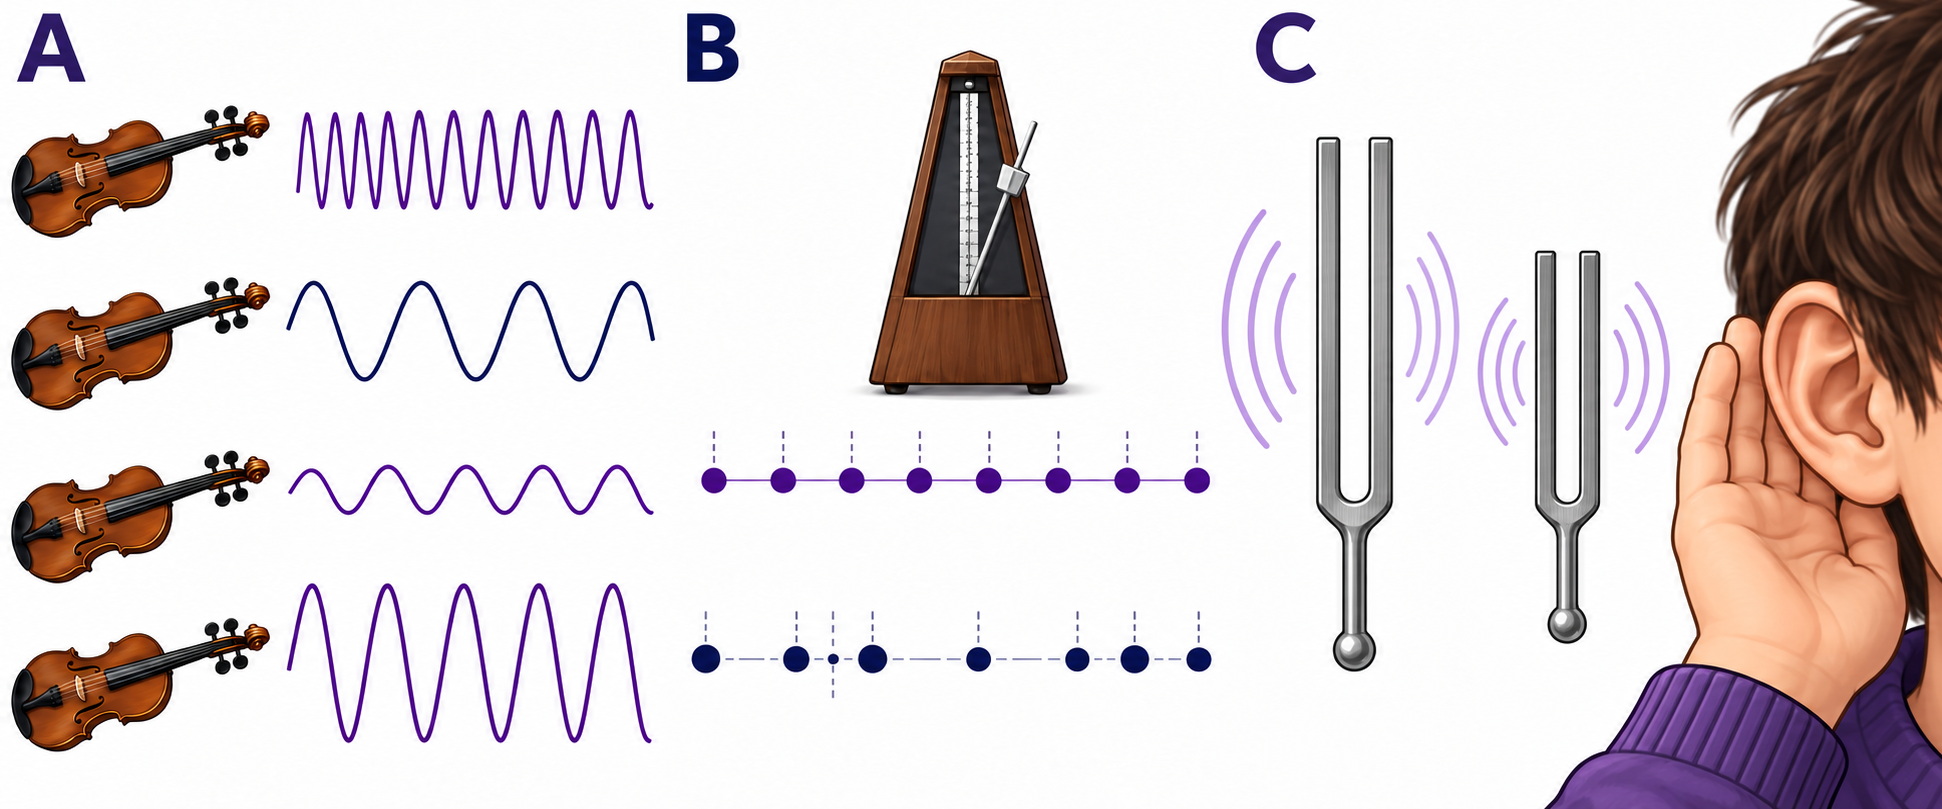
\includegraphics[width=\linewidth,height=0.26\textheight,keepaspectratio]{../assets/figure-f6141a0bb6d5.png}\par

{\small 本课重点看 C 区。A 比较振动疏密与振幅；B 稳定脉冲和节奏事件并不相同；C 两个音高之间可以比较方向与距离。波形仅作概念示意。}\par

{\footnotesize AI生成教学示意，非实物照片、原始史料或官方架构。生成方式：内置文生图；提示词见仓库 docs/image-prompts.json。}\end{center}

\Needspace{5\baselineskip}\section*{为什么“第三个”不等于“三个半音”}

以西方常用音名为例，从 C 到 E，按 C、D、E 连起止音一起计数，是三度；在十二平均律的键盘半音计数中则跨四个半音。[S5] 度数表达音名位置关系，半音数表达另一种距离。把两个计数法混用，会出现“为什么三度不是三个半音”的疑惑。

本课用西方常见乐理作为入门工具，不把它当作所有音乐文化的唯一标准。其他调律、装饰音和连续滑音不能全部用钢琴键之间的距离概括。图 C 的两个音叉只提示“比较两个音高”，不指定真实频率、音程或精确尺寸比例。

\Needspace{5\baselineskip}\section*{一个不需要识谱的实验}

轻声哼三次同一个音，再哼“低—高—低”三个音，最后哼“低—更高—低”。第一组以重复为主，后两组轮廓相同，但跨度可以不同。听起来相似不代表完全相同。

把你熟悉的一句旋律整体提高或降低到舒适位置，尽量保持各音之间的关系和时值。你仍能认出它，说明旋律识别依赖关系；但音色、节奏、歌词与记忆也有贡献，不能凭这个小实验得出“认歌只靠音程”的结论。它是观察练习，不是心理声学实验。

\Needspace{5\baselineskip}\section*{三分钟练习与自查}

选一个不超过十秒的熟悉乐句，用上箭头、下箭头、横线画出大致轮廓，并圈出你觉得跨度最大的位置。然后用一句话说明轮廓图没有记录什么。

参考：轮廓图没有准确记录每个音的高度、音程大小、节奏、音色或力度。能主动指出遗漏，比把草图当完整乐谱更重要。若你愿意扩展，可以对照 [S2] 的记谱入门，看看谱表如何补充一部分信息；今天无需学完整读谱规则。

\Needspace{5\baselineskip}\section*{复盘与明日连接}

旋律不仅由单个音构成，也由相邻声音的关系和时间展开构成。先听走向，再细看距离，能降低入门负担。明天学习乐句与呼吸：旋律在哪里像一句话结束，哪些停顿只是暂时悬念？

\Needspace{6\baselineskip}\section*{扩展学习 / Further reading}\small 以下为选读，不计入每日必做时间。\begin{enumerate}[leftmargin=1.6em]

\item [S1] \href{https://openstax.org/books/physics/pages/14-1-speed-of-sound-frequency-and-wavelength}{Speed of Sound, Frequency, and Wavelength} — 选读声音频率与音高的关系，公式推导可跳过。\par OpenStax | 发布：未标注 | 核验：2026-10-08

\item [S2] \href{https://openmusictheory.github.io/basicNotation.html}{Basic notation} — 认识音符、谱表和变音记号；本课不要求记住全部符号。\par Open Music Theory | 发布：未标注 | 核验：2026-10-08

\item [S3] \href{https://openmusictheory.github.io/rhythmicValues.html}{Rhythmic values} — 观察长短时值和休止符如何表达时间。\par Open Music Theory | 发布：未标注 | 核验：2026-10-08

\item [S4] \href{https://openmusictheory.github.io/meter.html}{Meter and time signatures} — 选看拍子分组与聆听示例；部分嵌入播放器可能需要额外登录。\par Open Music Theory | 发布：未标注 | 核验：2026-10-08

\item [S5] \href{https://openmusictheory.github.io/intervals.html}{Intervals and dyads} — 重点看半音数与音程度数不是同一种计数方法。\par Open Music Theory | 发布：未标注 | 核验：2026-10-08

\end{enumerate}

\end{document}